\documentclass{eecslides} 
\usepackage{amsmath}

%------------------------------

\title[Networks \& Biogeography]{Ecological networks in the anthropocene} 
\author[D. Gravel]{Dominique Gravel} 
\institute{UQAR -- Canada Research Chair in Biogeography and metacommunity ecology}
\website{http://www.chaire-eec.uqar.ca/} 
\date{\today}

\begin{document}

	\begin{frame}[plain] 
		\titlepage
	\end{frame}

%-------------------------------------------------------------------------------
%-------------------------------------------------------------------------------
	\section{Introduction}
%-------------------------------------------------------------------------------
%-------------------------------------------------------------------------------

	\begin{frame}
		\begin{center}
			\alert{\large{\textbf{We need a novel appproach to quantify biodiversity taking into account the diversity of ecological interactions}}}\\
		\end{center}	  	    
	\end{frame}

%-------------------------------------------------------------------------------

	\begin{frame}
		\begin{center}
		
\includegraphics[height=0.8\textheight]{earth}\\
		\end{center}
	\end{frame}

%-------------------------------------------------------------------------------

	\begin{frame}{Trends in biogeography}{Functional diversity}
		\begin{center}
		\includegraphics[height=0.7\textheight]{mouillot}\\
		\footnotesize{Mouillot et al. (2013)}
		\end{center}
	\end{frame}

%-------------------------------------------------------------------------------

	\begin{frame}{Trends in biogeography}{Phylogenetic diversity}
		\begin{center}
		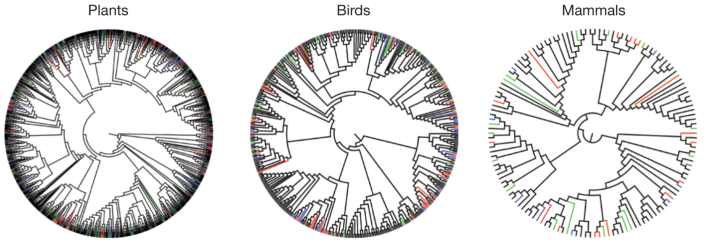
\includegraphics[height=0.45\textheight]{thuiller}\\
		\footnotesize{Thuiller et al. (2011)}\\
		\footnotesize{Mazel et al. (2014)}
		\end{center}
	\end{frame}

%-------------------------------------------------------------------------------

%	\begin{frame}{The rich history of community ecology}
%		\begin{center}
%		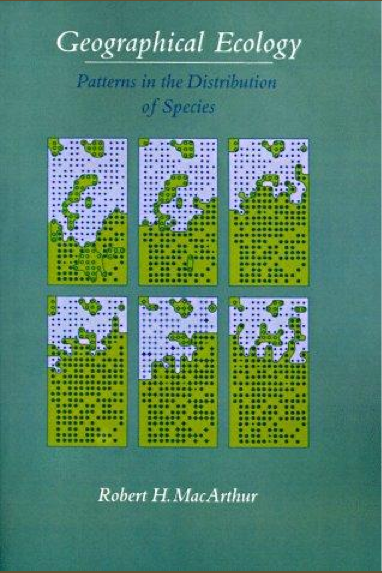
\includegraphics[height=0.7\textheight]{macarthur}\\
%		\end{center}
%	\end{frame}

%-------------------------------------------------------------------------------

	\begin{frame}
		\begin{center}
		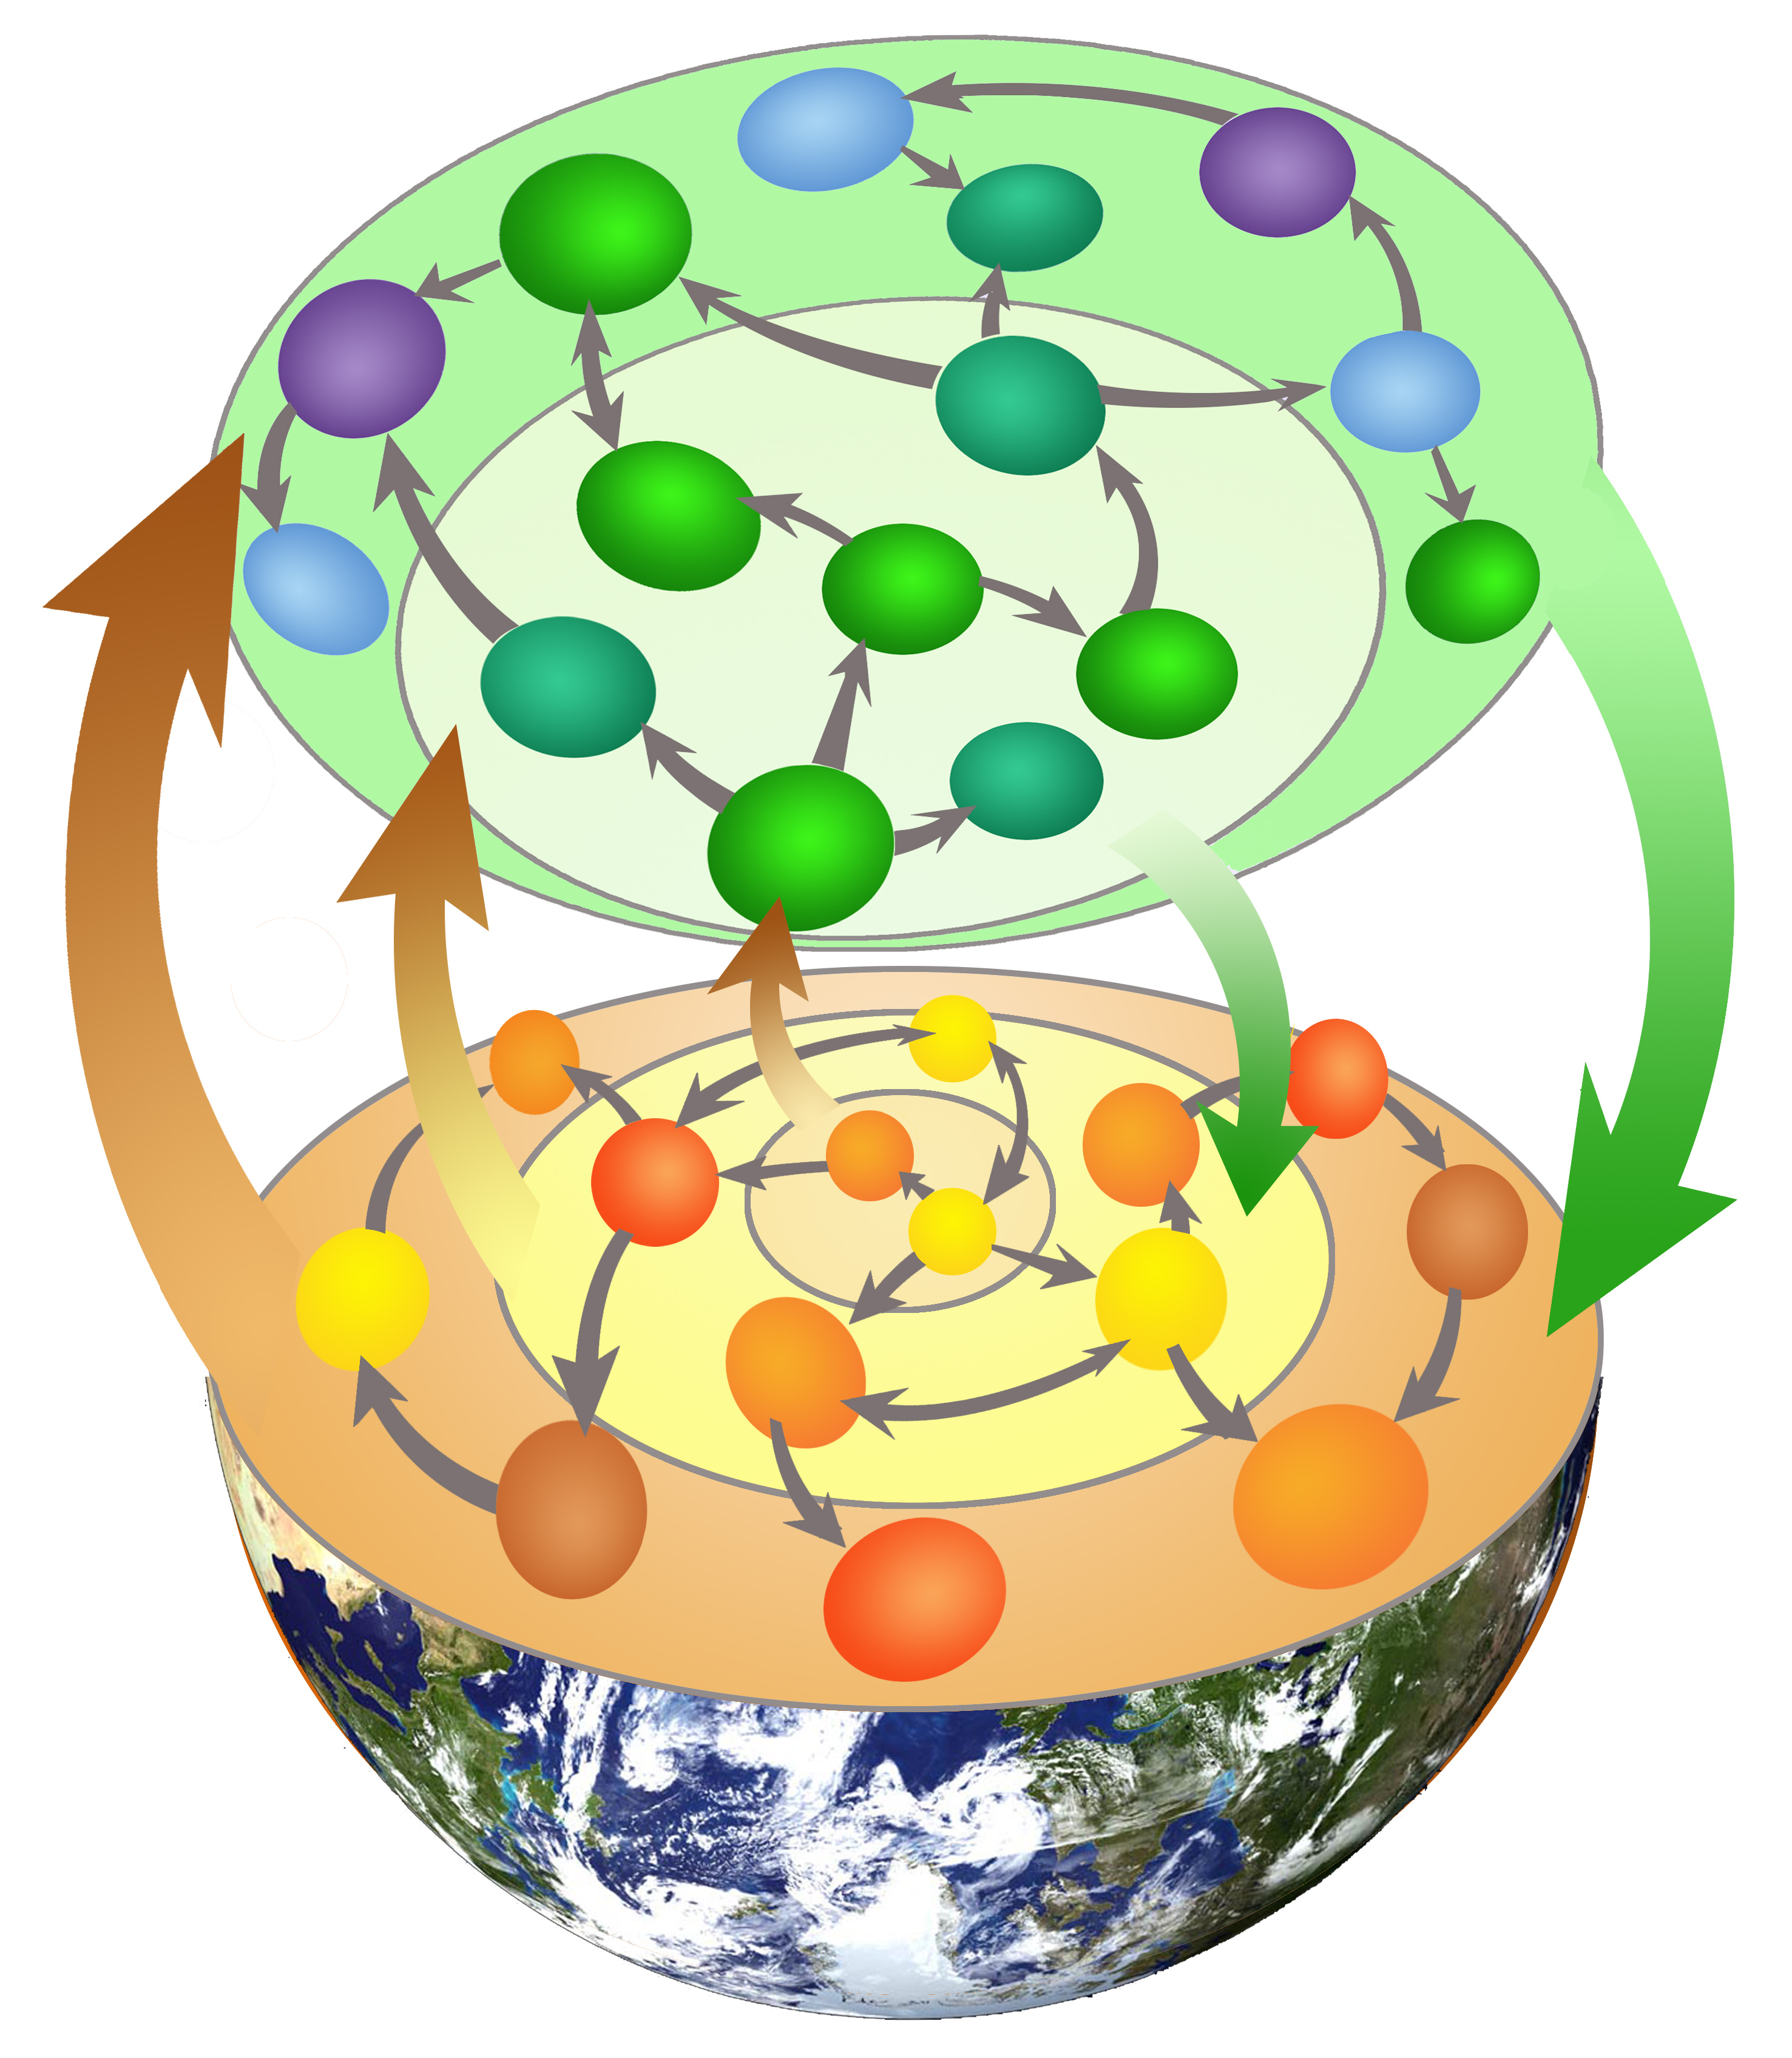
\includegraphics[height=0.85\textheight]{lab_logo}\\
		\end{center}	  	    
	\end{frame}

%-------------------------------------------------------------------------------
%-------------------------------------------------------------------------------
	\section{Networks}
%-------------------------------------------------------------------------------
%-------------------------------------------------------------------------------

	\begin{frame}{Communities are messy}
		\begin{center}
		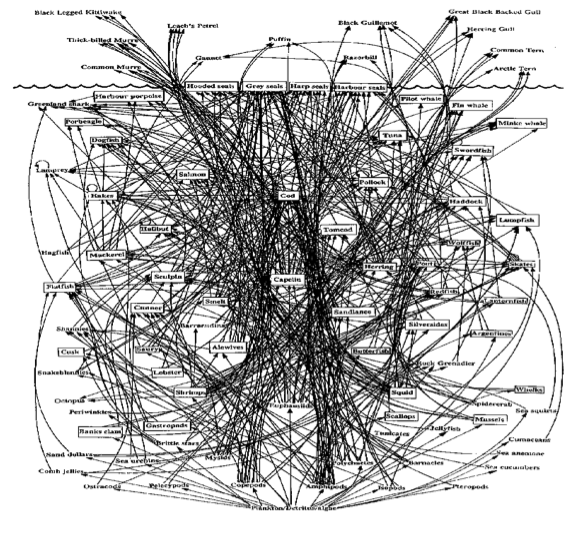
\includegraphics[height=0.65\textheight]{cod}\\
		\end{center}	
	\end{frame}

%-------------------------------------------------------------------------------

	\begin{frame}{Compressing information}
		\begin{center}
		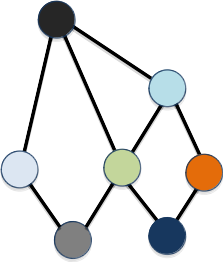
\includegraphics[height=0.5\textheight]{simple_network}\\
		\end{center}	
	\end{frame}

%-------------------------------------------------------------------------------

	\begin{frame}{A successfull program}{Phase 1}
		\begin{center}
		
\includegraphics[height=0.65\textheight]{may}\\
		\end{center}	
	\end{frame}

%-------------------------------------------------------------------------------

	\begin{frame}{A successfull program}{Phase 2}
		\begin{center}
		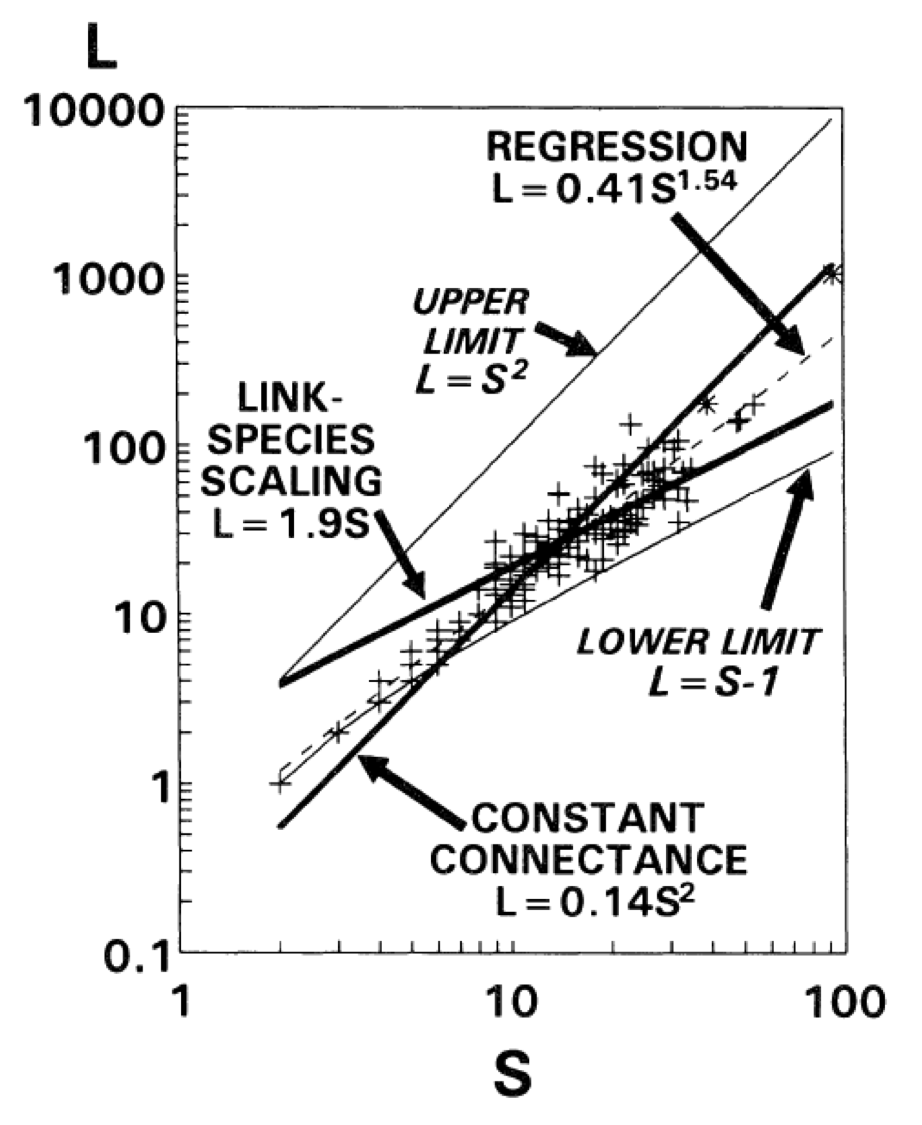
\includegraphics[height=0.65\textheight]{link_scaling}\\
		\footnotesize{Martinez (1992)}\\
		\end{center}	
	\end{frame}

%-------------------------------------------------------------------------------

	\begin{frame}{A successfull program}{Phase 3}
		\begin{center}
		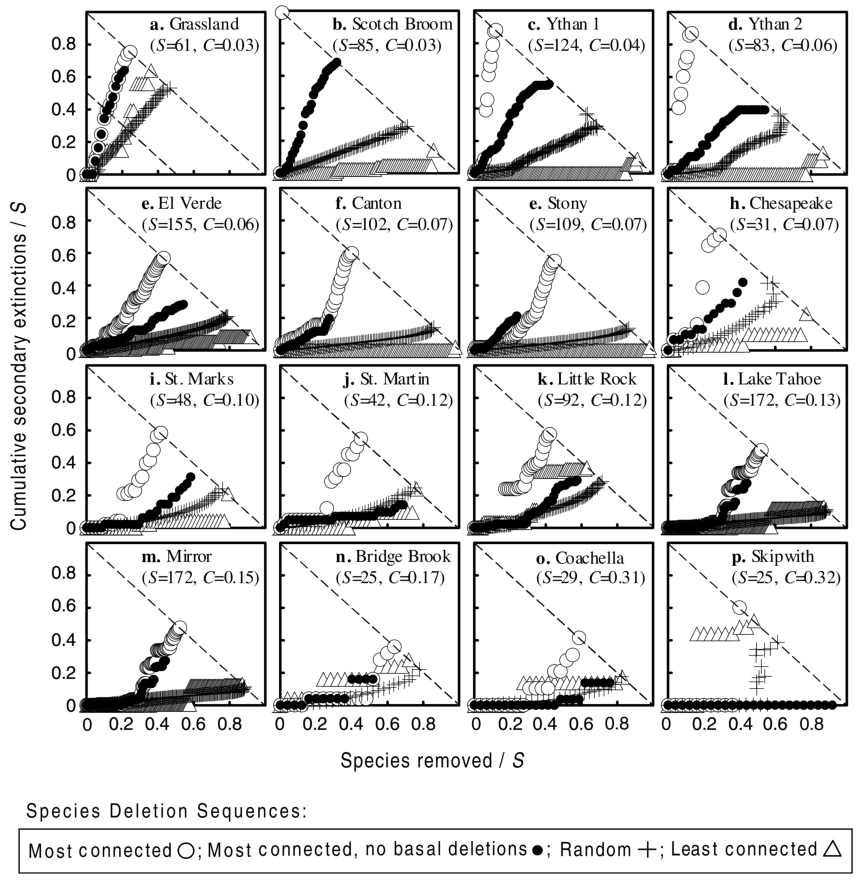
\includegraphics[height=0.65\textheight]{dunne}\\
		\footnotesize{Dunne et al. (2002)}\\
		\end{center}	
	\end{frame}

%-------------------------------------------------------------------------------

	\begin{frame}{But...}
		\begin{center}
			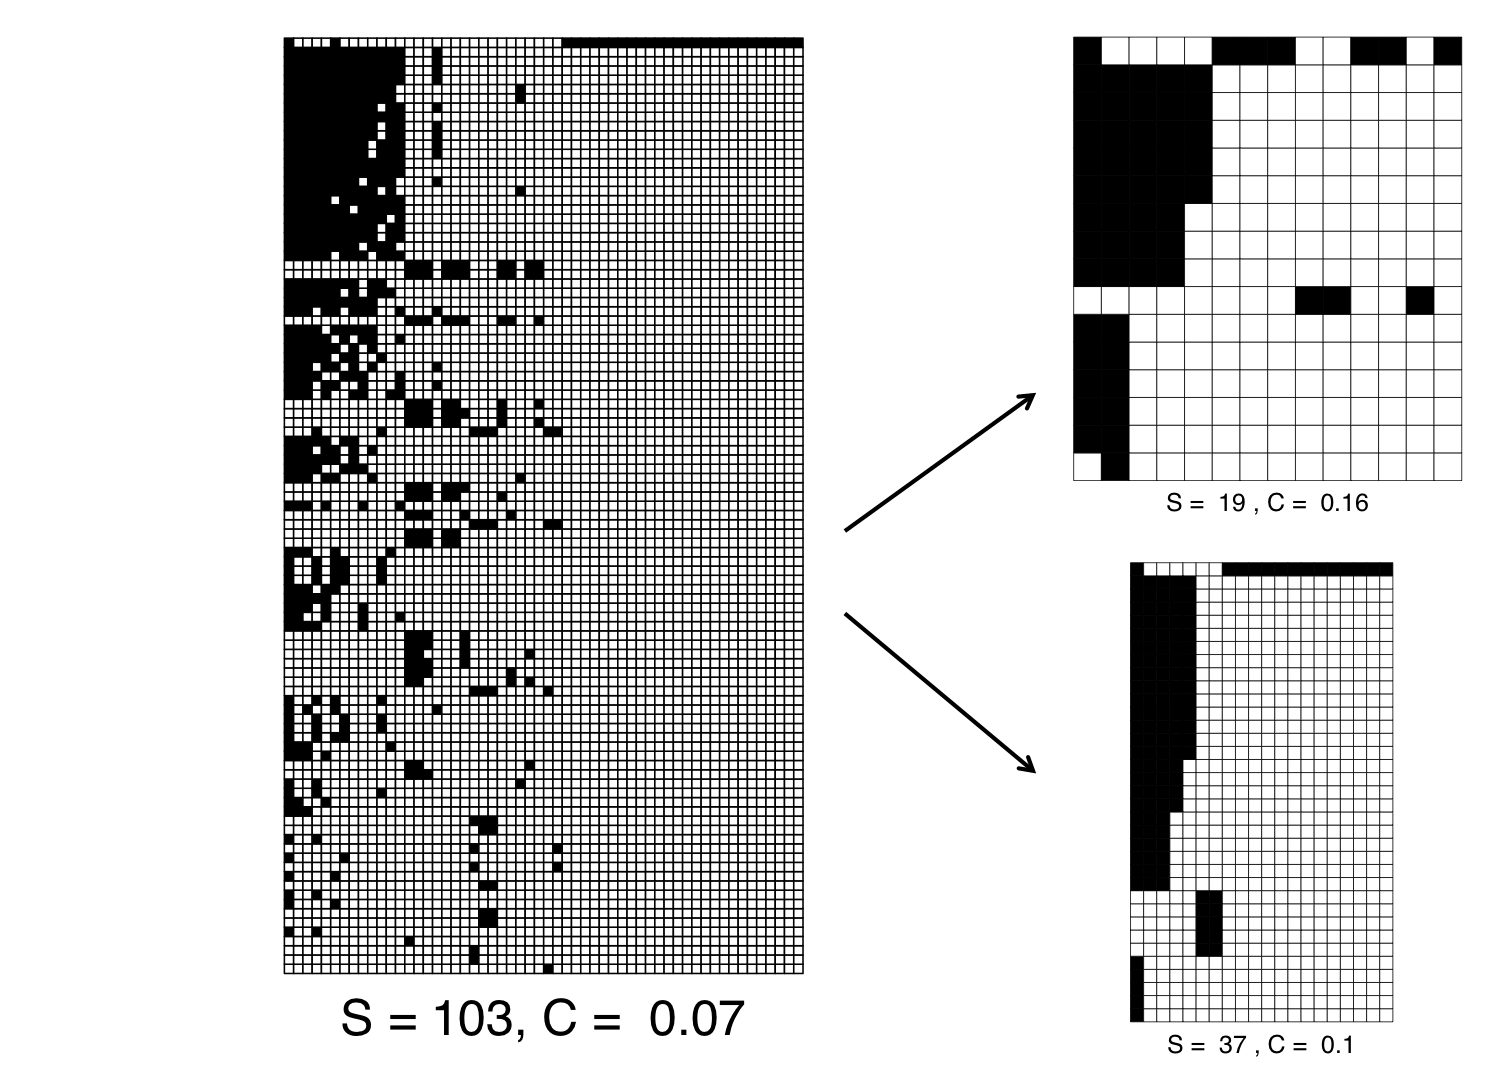
\includegraphics[height=0.55\textheight]{havens_sampling}\\
			\footnotesize{Gravel et al. (2011). \textit{Ecol. Lett.}}
		\end{center}   
		\begin{center}
			\alert{\textbf{What are the processes explaining how we move from a regional network (a metaweb) to a local community?}}
		\end{center}	 	    
	\end{frame}

%-------------------------------------------------------------------------------

	\begin{frame}{Biogeography of ecological interactions}
		\begin{center}
			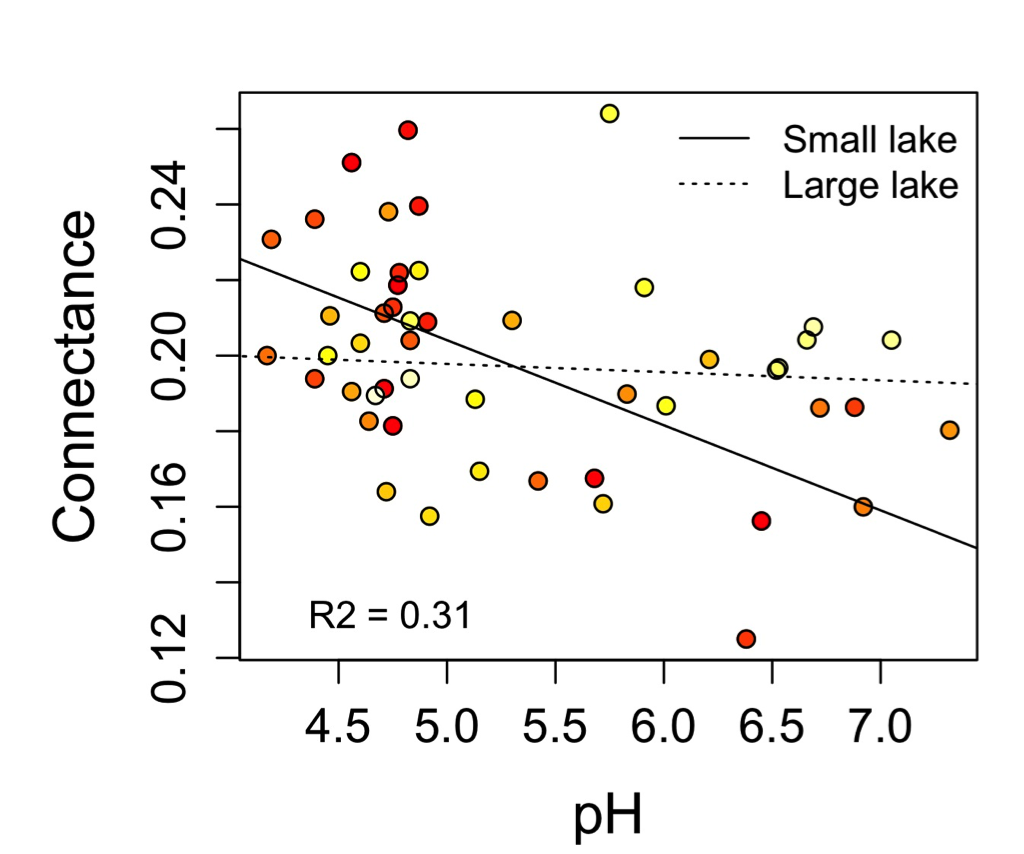
\includegraphics[height=0.6\textheight]{havens_ph}
		\end{center}   
	\end{frame}

%-------------------------------------------------------------------------------

	\begin{frame}{Spatial variation of interaction networks}
		\begin{center}
			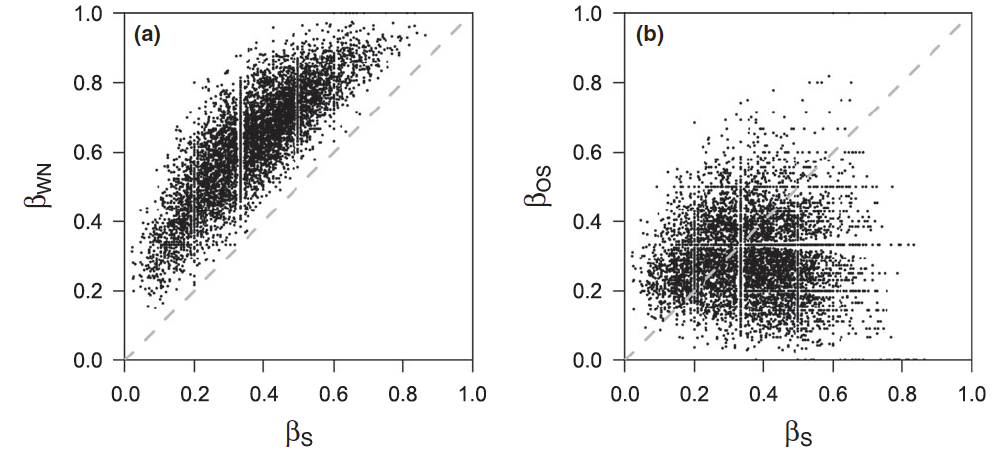
\includegraphics[height=0.45\textheight]{poisot2012}\\
			\footnotesize{Poisot et al. (2012). \textit{Ecol. Lett.}}
		\end{center} 
		Networks do vary in space because of:
			\begin{itemize}
				\item Species turnover;
				\item Link turnover;
			\end{itemize}	
		The variation of network structure is independent of the variation in species composition	      
	\end{frame}

%-------------------------------------------------------------------------------

%	\begin{frame}{The determinism of network models}
%		\begin{itemize}
%			\item Random networks
%			\item Cascade \& Generalized cascade
%			\item Niche model, Minimal potential niche model \& Probabilistic niche model
%			\item Nested hierarchy
%			\item \textit{Neutral networks}
%		\end{itemize}  
%	\end{frame}

%-------------------------------------------------------------------------------
%-------------------------------------------------------------------------------
	\section{The niche}
%-------------------------------------------------------------------------------
%-------------------------------------------------------------------------------

	\begin{frame}{Variation in community structure}{The niche}
		\begin{center}
			\textit{\alert{[The niche is] the joint description of the environmental conditions that allow a species to satisfy its minimum requirements so that the birth rate of a local population is equal or greater than its death rate along with the set of per capita effects of that species on these environmental conditions.}} (Chase and Leibold, 2003)
		\end{center}
		
	\end{frame}

%-------------------------------------------------------------------------------

	\begin{frame}{The Grinnellian niche}
		\begin{center}
		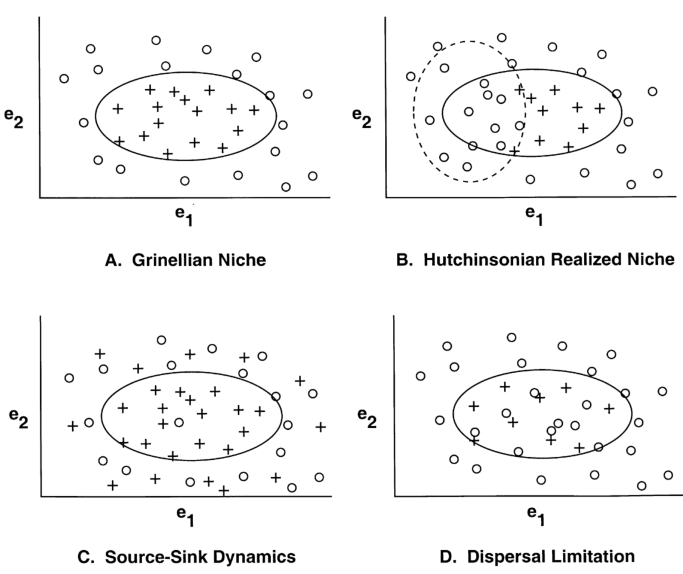
\includegraphics[height=0.6\textheight]{pulliam}\\
		\footnotesize{Pulliam (2000)}
		\end{center}
	\end{frame}

%-------------------------------------------------------------------------------

	\begin{frame}{The Eltonian niche}
		\begin{center}
		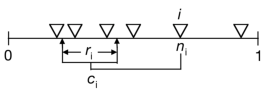
\includegraphics[height=0.35\textheight]{martinez}\\
		\footnotesize{Williams \& Martinez (2000)}
		\end{center}
	\end{frame}

%-------------------------------------------------------------------------------

%	\begin{frame}{Mapping ecological networks}
%		\begin{center}
%		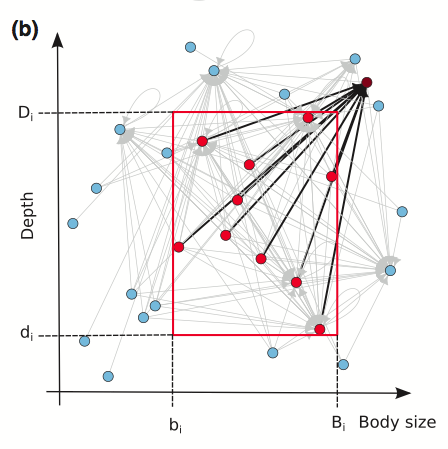
\includegraphics[height=0.6\textheight]{eklof}\\
%		\footnotesize{Eklof et al (2013)}
%		\end{center}
%	\end{frame}

%-------------------------------------------------------------------------------

	\begin{frame}{Mapping an integrated niche}
		\begin{center}
		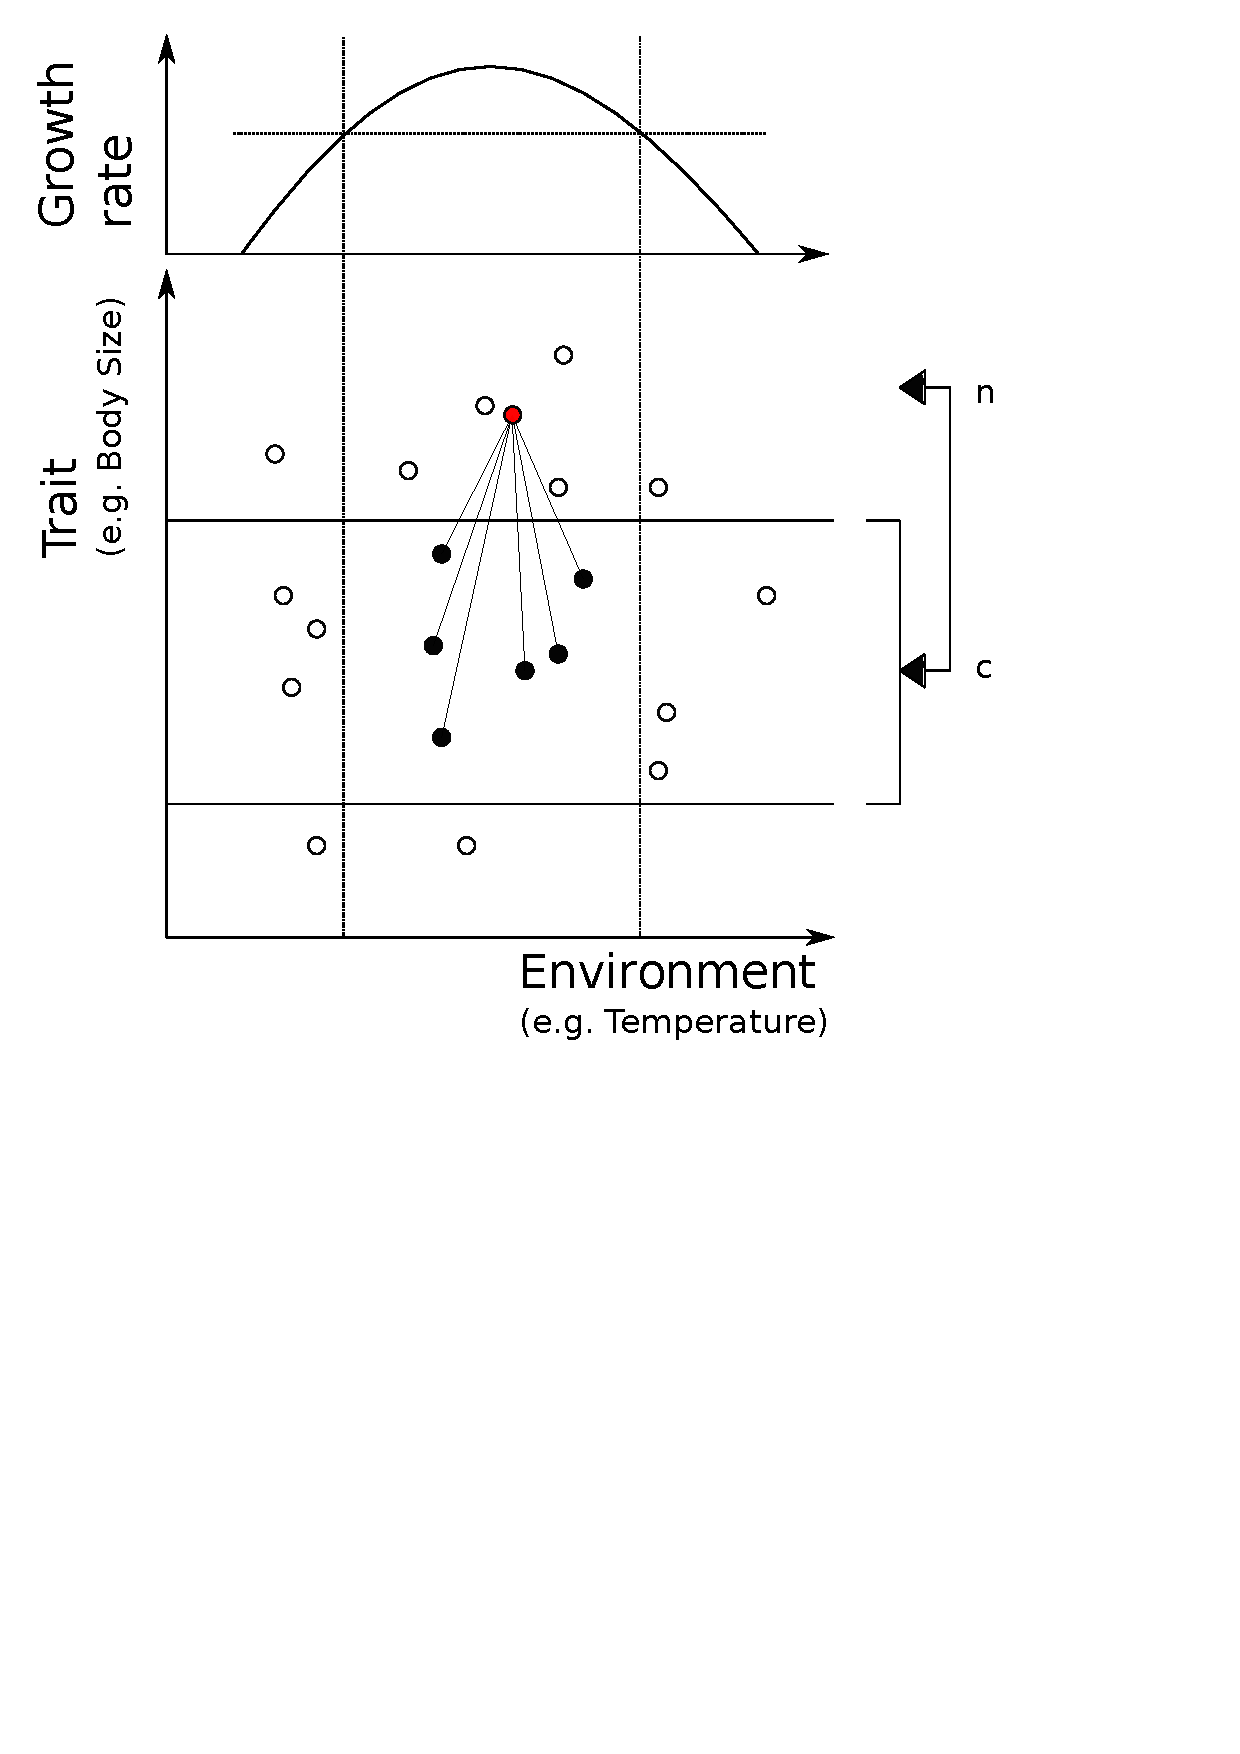
\includegraphics[height=1.2\textheight]{integrated_niche}\\
		\end{center}
	\end{frame}

%-------------------------------------------------------------------------------

	\begin{frame}{Framework}{Formulating network sampling as a stochastic process}
	Define the stochastic variable $X_{ix}$ representing the occurrence of species $i$ in a local community $x$. \\
	\vskip 1em

	And the variable $L_{ijx}$ representing the occurrence of an interaction between species $i$ and $j$ at location $x$.	
	\vskip 1em

	We are looking for the probability that an interaction occurs:
		\begin{center}
			$P(L_{ijx} = 1,X_{ix} = 1,X_{jx} = 1)$
		\end{center}	

	\end{frame}

%-------------------------------------------------------------------------------

	\begin{frame}{Conditional probabilities}
	Obtained from the product rule we get:
		\begin{center}
			$P(L_{ijx},X_{ix},X_{jx}) = P(L_{ijx}|X_{ix},X_{jx})P(X_{ix},X_{jx})$
		\end{center}
	Where:\\
	$P(L_{ijx}|X_{ix},X_{jx})$ is the metaweb (the Eltonian niche)\\
 	$P(X_{ix},X_{jx})$ is the co-occurrence matrix (the Grinnellian niche)
		
	\end{frame}

%-------------------------------------------------------------------------------

	\begin{frame}{Variants}
	 We could refine the model with the addition of a condition on the environment, such as:
		\begin{center}
			$P(L_{ijx}|X_{ix},X_{jx},E_x)$\\
			and\\
			$P(X_{ix},X_{jx}|E_x)$
		\end{center}   
	We could also specify neutral dynamics underlying community assembly:
 		\begin{center}
			$P(X_{ix},X_{jx}|E_x) =P(X_{ix}|E_x)P(X_{jx}|E_x)$
		\end{center}   
	\end{frame}

%-------------------------------------------------------------------------------

	\begin{frame}{Example}{Tropical cavity-nesting bees and wasps and their parasitoids}
	    
	From \textit{Tylianakis et al. 2007. Habitat modification alters the structure of tropical host-parasitoid food webs. Nature, 44:202-205}
	\begin{columns}
		\begin{column}{0.7\textwidth}			
			\begin{itemize}
				\item 48 networks, 4 090 recorded interactions
				\item 5 habitats: forest, abandoned coffee agroforest, coffee agroforest, pasture, rice
				\item 33 species of bees and wasps (Hymenoptera: Apidae, Megachilidae, Mutilidae, Pompilidae, Sphecidae, Vespidae)
				\item 9 parasitoid and kleptoparasite (Hymenoptera: Eulophidae, Ichneumonidae, Leucospidae, Megachilidae and Chrysididae; Dyptera: Bombyliidae)
			\end{itemize}

		\end{column}

%----
		\begin{column}{0.3\textwidth}
			\begin{center}
				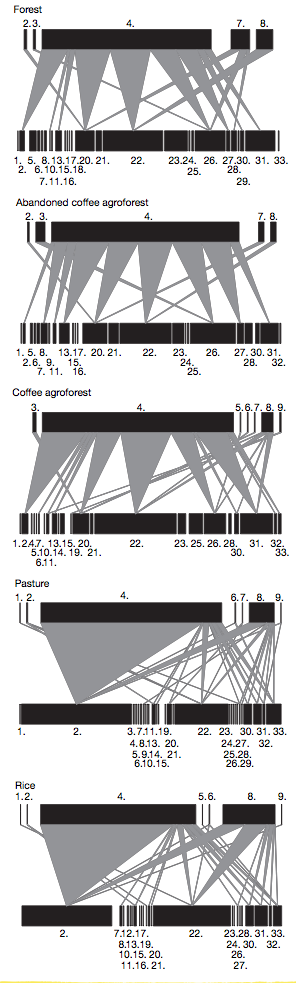
\includegraphics[height=0.65\textheight]{tylianakis}\\
			\end{center}
		\end{column}				
	\end{columns}	   
	\end{frame}

%-------------------------------------------------------------------------------

	\begin{frame}{Example}{Network \#34, Pasture}
		\begin{center}
			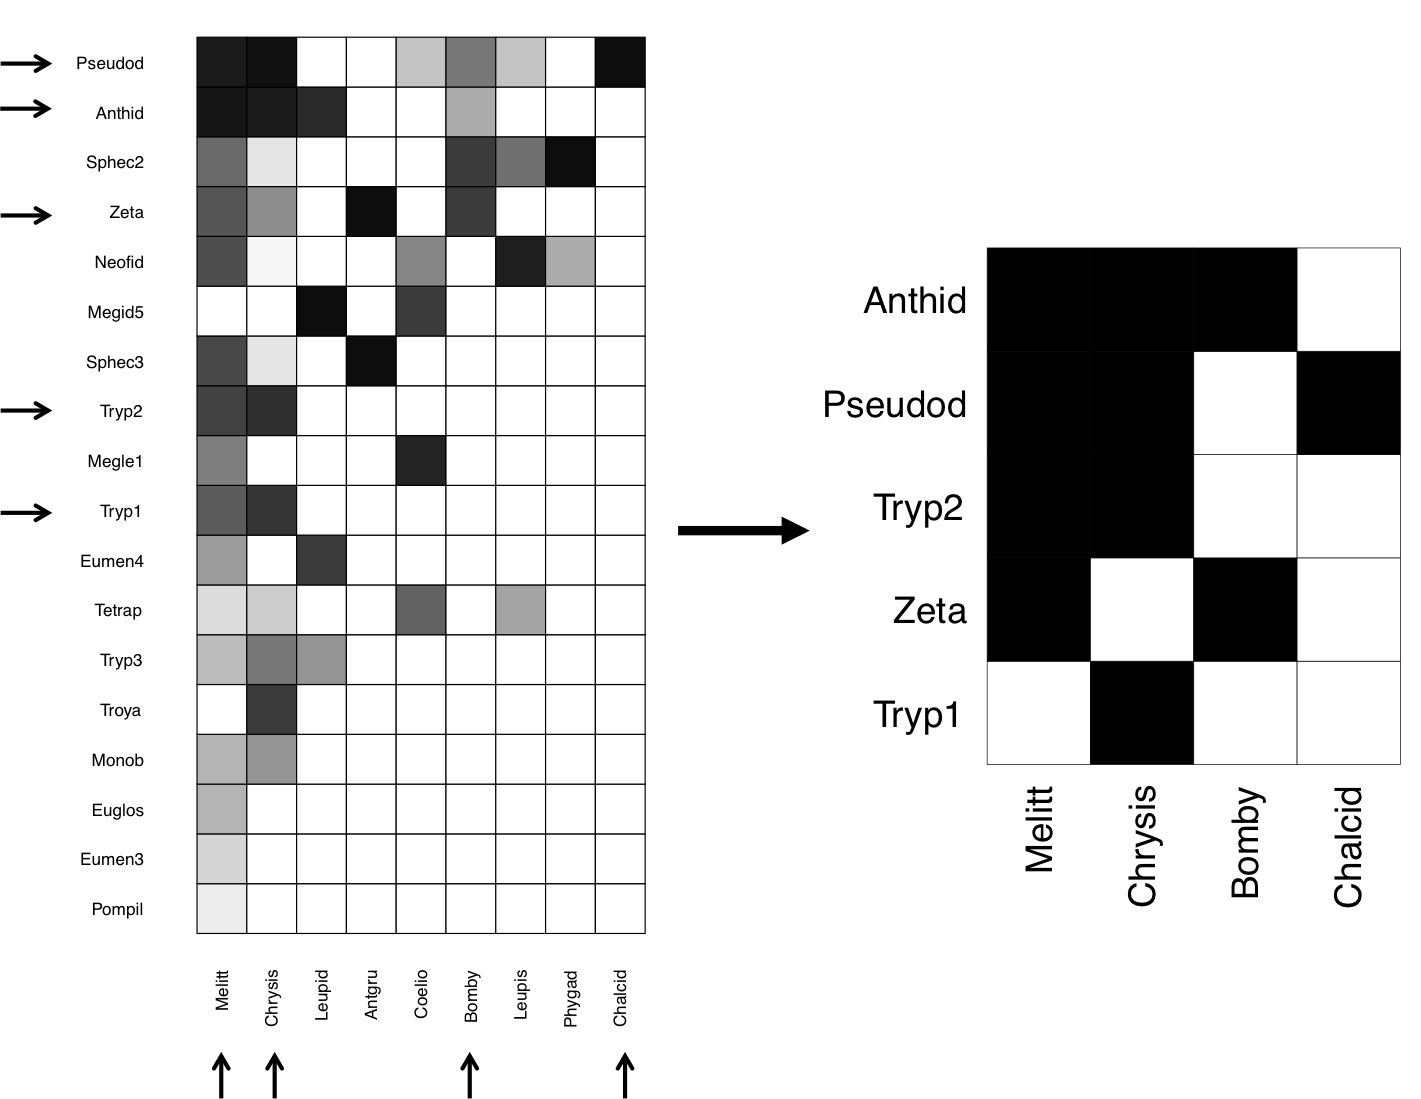
\includegraphics[height=0.75\textheight]{example}\\
		\end{center}
	\end{frame}

%-------------------------------------------------------------------------------

	\begin{frame}{Example}{Observed vs Predicted}
		\begin{tabular}{lll}
			\hline
			\textbf{Interpretation} & \textbf{Model} & \textbf{$L(H|D)$}\\
			\hline
			\textit{Basic model} & &\\
			No effect of E & $P(L_{ijx}|X_{ix},X_{jx})P(X_{ix},X_{jx})$ & -19.36\\
			\\
			\textit{Metaweb definitions} & & \\
			Conditional on E & $P(L_{ijx}|X_{ix},X_{jx}|E_x)P(X_{ix},X_{jx})$ & -10.37\\
			Aggregated metaweb & $P(L^*_{ijx}|X_{ix},X_{jx})P(X_{ix},X_{jx})$ & -27.96\\
			\\
			\textit{Co-occurrence} & &\\
			Neutral assembly & $P(L_{ijx}|X_{ix},X_{jx})P(X_{ix})P(X_{jx})$ &  -20.15\\
			Conditional on E& $P(L_{ijx}|X_{ix},X_{jx})P(X_{ix}|E_x)P(X_{jx}|E_x)$ & -13.30\\
			\hline
		\end{tabular}
	\end{frame}

%-------------------------------------------------------------------------------

	\begin{frame}{Summary of the key ideas}
		\begin{itemize}
			\item Networks are not deterministic
			\item Links do change with the environment
			\item The environment also affect species turnover and thus network turnover
			\item Very weak effect of non-random species associations on the variation of network structure
		\end{itemize}
	\end{frame}

%-------------------------------------------------------------------------------
%-------------------------------------------------------------------------------
	\section{Application}
%-------------------------------------------------------------------------------
%-------------------------------------------------------------------------------

	\begin{frame}{Application}{Inferring the metaweb from traits}
	 The problem: inferring interactions from species that never co-occurred and will be found in novel assemblages 
	\end{frame}

%-------------------------------------------------------------------------------

	\begin{frame}{Application}{Inferring the metaweb from traits}
		\begin{center}
			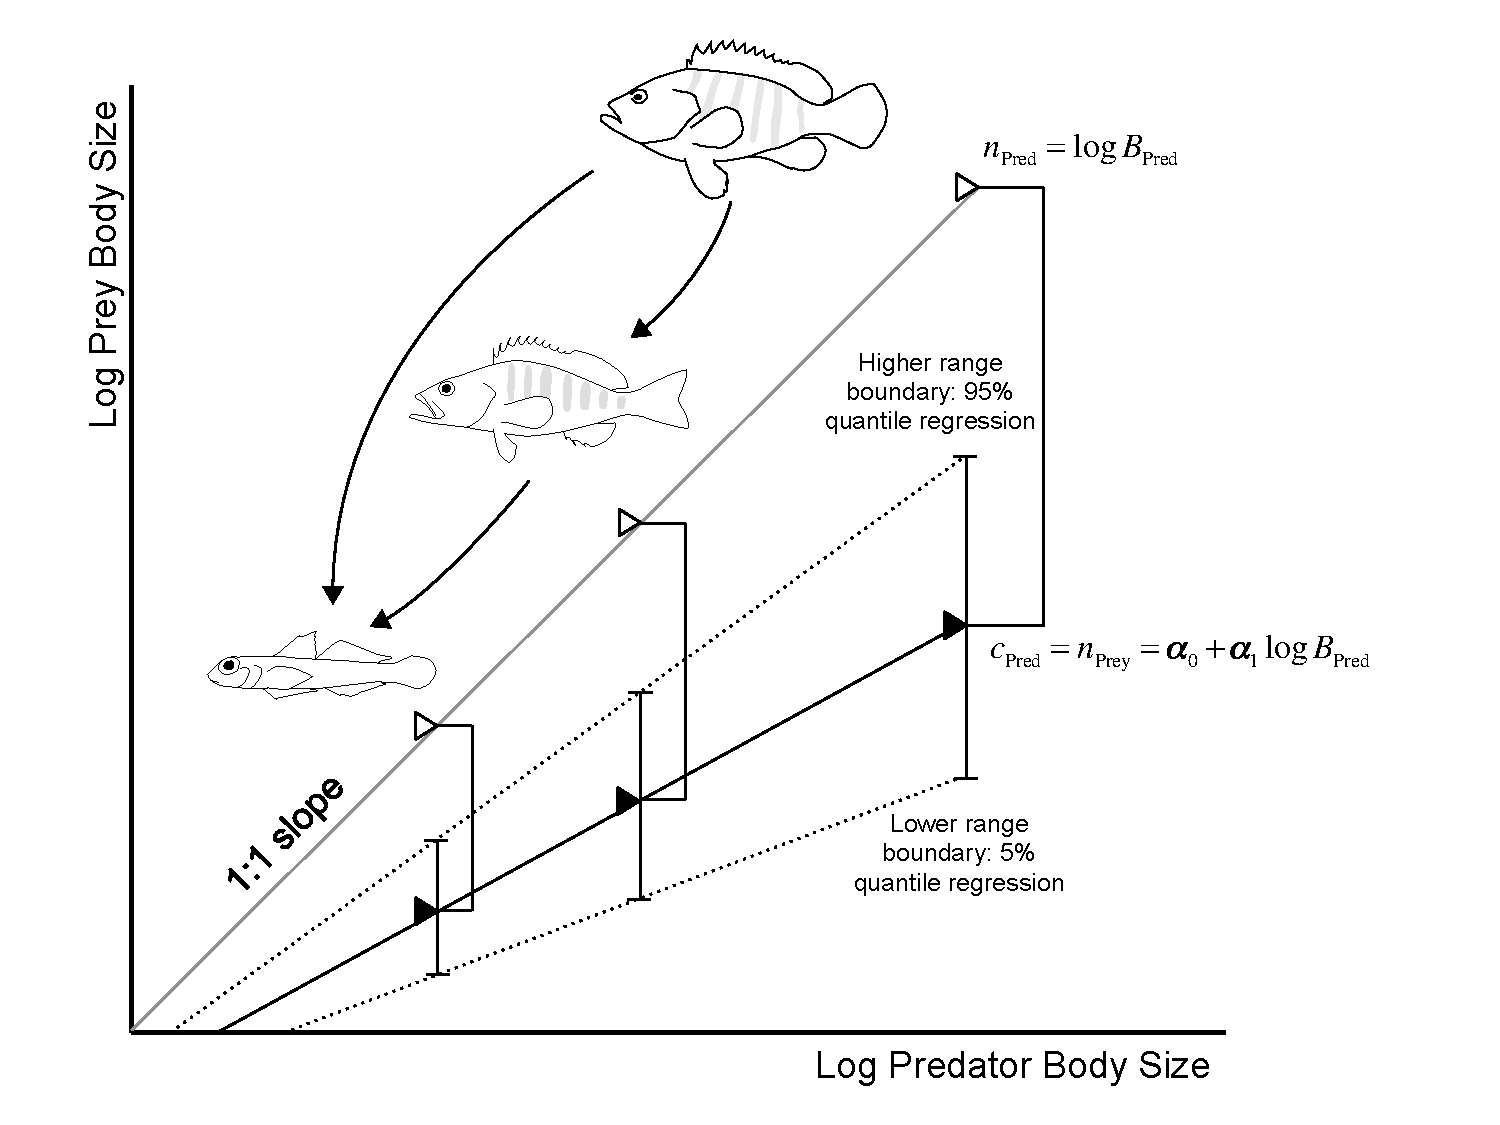
\includegraphics[height=0.55\textheight]{fig_MEE}\\
			\footnotesize{Gravel et al. (2013). \textit{Meth. Ecol. Evol.}}
		\end{center}
	\end{frame}

%-------------------------------------------------------------------------------

	\begin{frame}{Application}{Pelagic food web of the Mediterranean sea}
	Without information on the probability of interactions, we considered a metweb \textit{à la Havens} and neutral co-occurrence:\\	    
		\begin{center}
			$P(L_{ijx},X_{ix},X_{jx}|E_x) = P(L_{ijx}|X_{ix},X_{jx})P(X_{ix}|E_x)P(X_{jx}|E_x)$
		\end{center}
		\begin{center}
			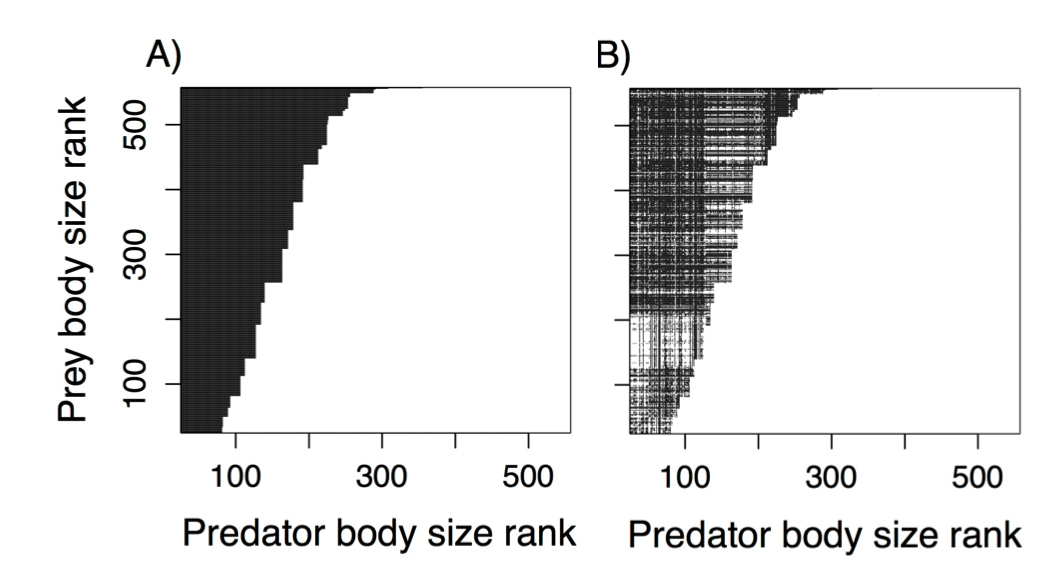
\includegraphics[height=0.5\textheight]{Example_MED}\\
			\footnotesize{Gravel et al. (2013)}
		\end{center}
	\end{frame}

%-------------------------------------------------------------------------------

	\begin{frame}{Application}{Pelagic food web of the Mediterranean sea}	  
		\begin{center}
			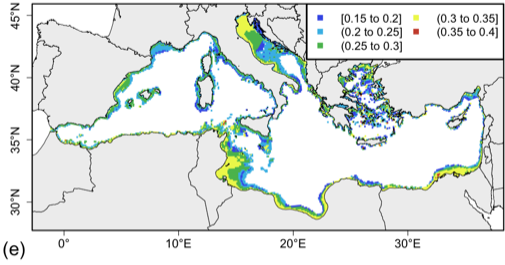
\includegraphics[height=0.35\textheight]{med_present}\\
			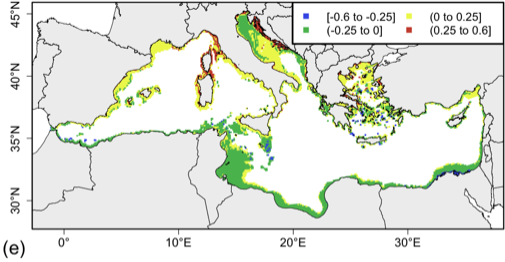
\includegraphics[height=0.35\textheight]{med_future}\\
			\footnotesize{Albouy et al. (2014)}
		\end{center}
	\end{frame}

%-------------------------------------------------------------------------------

	\begin{frame}{Application}{Pelagic food web of the Mediterranean sea}	  
		\begin{center}
			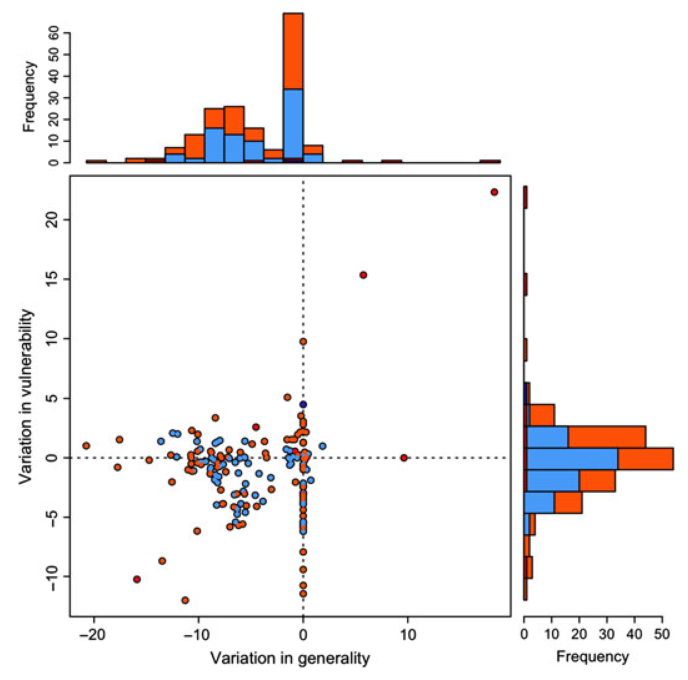
\includegraphics[height=0.6\textheight]{Albouy2014}\\
			\footnotesize{Albouy et al. (2014)}
		\end{center}
	\end{frame}
	
%-------------------------------------------------------------------------------
%-------------------------------------------------------------------------------
	\section{Conclusion}
%-------------------------------------------------------------------------------
%-------------------------------------------------------------------------------

	\begin{frame}{Conclusion}{A new perspective to community structure}
		\begin{center}
		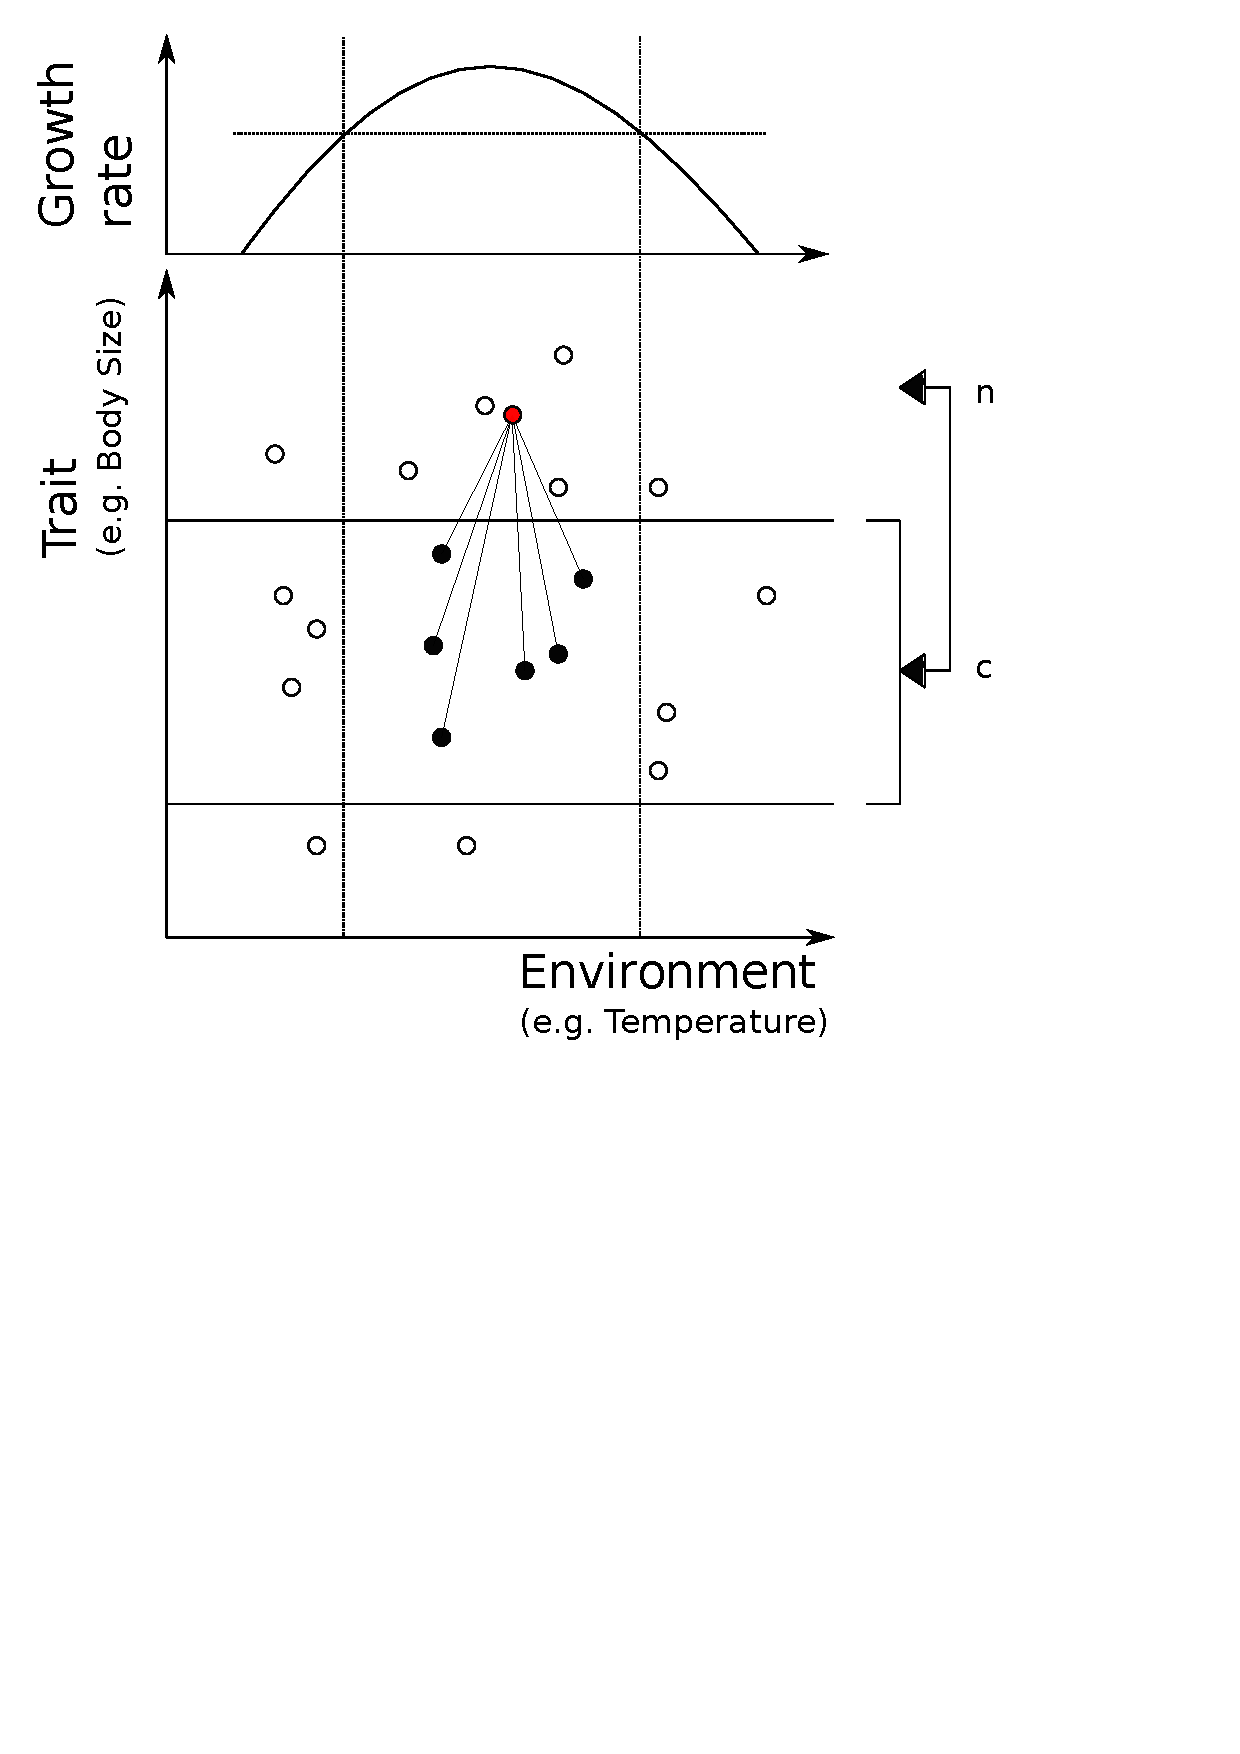
\includegraphics[height=1.2\textheight]{integrated_niche}\\
%		$P(L_{ijx},X_{ix},X_{jx}) = P(L_{ijx}|X_{ix},X_{jx})P(X_{ix},X_{jx})$
		\end{center}
	\end{frame}

%-------------------------------------------------------------------------------

	\begin{frame}{Future developments}{Inverse species distribution modelling}
	Given a theory for species co-occurrence, we could re-arrange information:\\
		\begin{align*}
			P(L_{ijx},X_{ix},X_{jx}|E_x) &= P(L_{ijx}|X_{ix},X_{jx},E_x)P(X_{ix},X_{jx}|E_x)\\
			&= P(L_{ijx}|X_{ix},X_{jx},E_x)P(X_{ix}|X_{jx},E_x)P(X_{jx}|E_x)\\
		\end{align*}
	And invert it to derive a probability of species occurrence, accounting for the environment and interactions: 		    
		\begin{center}
			$P(X_{jx}|E_x)=\frac{P(L_{ijx}|X_{ix},X_{jx},E_x)P(X_{ix}|X_{jx},E_x)}{P(L_{ijx},X_{ix},X_{jx}|E_x)}$
		\end{center}
	\end{frame}



%------------------------------
	\begin{frame}{Acknowledgements}
	    
	\textbf{Co-authors:} Range limits working group, Timothée Poisot, Camille Albouy, Jason
	Tylianakis, Daniel Stouffer, Jennifer Dunne, SFI, David Mouillot,
	Working group on gradient-based network research;\\ 
	\vskip 1em
	\textbf{Funding:} NSERC, FRQNT, Canada Research Chair program, Quebec
	Center for Biodiversity Sciences, Santa Fe Institute, UQAR.

	\end{frame}

%------------------------------



\end{document}
